\documentclass[11pt]{article}
% Shared preamble of the RMC kernel write-ups (% Shared preamble of the RMC kernel write-ups (% Shared preamble of the RMC kernel write-ups (\input{preamble} after \documentclass).
\usepackage[margin=1in]{geometry}
\usepackage{amsmath,amssymb,bm}
\usepackage{graphicx}
\usepackage{booktabs}
\usepackage{hyperref}

\newcommand{\dd}{\,\mathrm{d}}
\newcommand{\Ein}{E}
\newcommand{\Eout}{E'}
\newcommand{\Ecm}{E_{c}}
\newcommand{\mucm}{\mu_{c}}
\newcommand{\mulab}{\mu_0}

% Common closing section: how the verification figures are produced
\newcommand{\verificationmethod}{%
Each figure is produced by \texttt{verification/verify\_laws.py}. For an incident
energy $\Ein$ along $+z$, $10^6$ collisions are sampled with MC/DC's own reaction
sampler (\texttt{sample\_elastic\_scattering}, \texttt{sample\_inelastic\_scattering}
or \texttt{sample\_fission}), and every emitted neutron is histogrammed in
$48 \times 24$ bins of $(\Eout, \mulab)$, with $\mulab$ the lab cosine to $+z$. The
inverted kernel used by RMC is integrated over the same bins (Gauss--Legendre panels;
two-body lines are split where $\mulab^*(\Eout)$ crosses a cosine edge), multiplied by
the number of collisions, and compared with a $\chi^2$ test over bins with at least 5
expected counts (the rest pooled into one bin). The tables list $\chi^2/\mathrm{dof}$,
its $p$-value, the emitted neutrons per collision (sampled vs.\ the integral of the
inverted kernel), and the largest relative change of a bin integral when the
quadrature panels are doubled. Left panels: outgoing-energy marginal; middle:
lab-cosine marginal; right: per-bin $z = (\text{sampled} - \text{inverted}) /
\sqrt{\text{inverted}}$.}
 after \documentclass).
\usepackage[margin=1in]{geometry}
\usepackage{amsmath,amssymb,bm}
\usepackage{graphicx}
\usepackage{booktabs}
\usepackage{hyperref}

\newcommand{\dd}{\,\mathrm{d}}
\newcommand{\Ein}{E}
\newcommand{\Eout}{E'}
\newcommand{\Ecm}{E_{c}}
\newcommand{\mucm}{\mu_{c}}
\newcommand{\mulab}{\mu_0}

% Common closing section: how the verification figures are produced
\newcommand{\verificationmethod}{%
Each figure is produced by \texttt{verification/verify\_laws.py}. For an incident
energy $\Ein$ along $+z$, $10^6$ collisions are sampled with MC/DC's own reaction
sampler (\texttt{sample\_elastic\_scattering}, \texttt{sample\_inelastic\_scattering}
or \texttt{sample\_fission}), and every emitted neutron is histogrammed in
$48 \times 24$ bins of $(\Eout, \mulab)$, with $\mulab$ the lab cosine to $+z$. The
inverted kernel used by RMC is integrated over the same bins (Gauss--Legendre panels;
two-body lines are split where $\mulab^*(\Eout)$ crosses a cosine edge), multiplied by
the number of collisions, and compared with a $\chi^2$ test over bins with at least 5
expected counts (the rest pooled into one bin). The tables list $\chi^2/\mathrm{dof}$,
its $p$-value, the emitted neutrons per collision (sampled vs.\ the integral of the
inverted kernel), and the largest relative change of a bin integral when the
quadrature panels are doubled. Left panels: outgoing-energy marginal; middle:
lab-cosine marginal; right: per-bin $z = (\text{sampled} - \text{inverted}) /
\sqrt{\text{inverted}}$.}
 after \documentclass).
\usepackage[margin=1in]{geometry}
\usepackage{amsmath,amssymb,bm}
\usepackage{graphicx}
\usepackage{booktabs}
\usepackage{hyperref}

\newcommand{\dd}{\,\mathrm{d}}
\newcommand{\Ein}{E}
\newcommand{\Eout}{E'}
\newcommand{\Ecm}{E_{c}}
\newcommand{\mucm}{\mu_{c}}
\newcommand{\mulab}{\mu_0}

% Common closing section: how the verification figures are produced
\newcommand{\verificationmethod}{%
Each figure is produced by \texttt{verification/verify\_laws.py}. For an incident
energy $\Ein$ along $+z$, $10^6$ collisions are sampled with MC/DC's own reaction
sampler (\texttt{sample\_elastic\_scattering}, \texttt{sample\_inelastic\_scattering}
or \texttt{sample\_fission}), and every emitted neutron is histogrammed in
$48 \times 24$ bins of $(\Eout, \mulab)$, with $\mulab$ the lab cosine to $+z$. The
inverted kernel used by RMC is integrated over the same bins (Gauss--Legendre panels;
two-body lines are split where $\mulab^*(\Eout)$ crosses a cosine edge), multiplied by
the number of collisions, and compared with a $\chi^2$ test over bins with at least 5
expected counts (the rest pooled into one bin). The tables list $\chi^2/\mathrm{dof}$,
its $p$-value, the emitted neutrons per collision (sampled vs.\ the integral of the
inverted kernel), and the largest relative change of a bin integral when the
quadrature panels are doubled. Left panels: outgoing-energy marginal; middle:
lab-cosine marginal; right: per-bin $z = (\text{sampled} - \text{inverted}) /
\sqrt{\text{inverted}}$.}


\title{Inverted kernels: tabulated and multi-table distributions (ENDF Law 4),
tabulated angles, and fission spectra}
\date{}

\begin{document}
\maketitle

\noindent Code: \texttt{evaluate\_tabulated}, \texttt{evaluate\_multi\_table} in
\texttt{mcdc/rmc/evaluate.py}; \texttt{\_emission\_density},
\texttt{continuous\_lab\_density} in \texttt{mcdc/rmc/reaction.py}.

\section{Tabulated distribution}

\texttt{sample\_tabulated} draws $\xi$, finds the CDF interval $[c_k, c_{k+1})$ and
inverts the segment exactly for a histogram PDF ($p = p_k$) or a linear PDF
($p = p_k + m(x - x_k)$, a quadratic CDF). Exact inversion of the CDF means the sampled
density is the table itself:
\begin{equation}
  p(x) = p_k \quad\text{or}\quad p(x) = p_k + \frac{p_{k+1}-p_k}{x_{k+1}-x_k}(x - x_k),
  \qquad x_k \le x < x_{k+1},
\end{equation}
and zero outside $[x_1, x_K]$ (the PDF values are normalized by MC/DC at load time).

\section{Multi-table distribution}

For an incident grid $E_i \le \Ein < E_{i+1}$, $f = (\Ein - E_i)/(E_{i+1}-E_i)$, the
sampler uses table $i$ with probability $1-f$ and table $i+1$ with probability $f$
(stochastic interpolation); off the grid only the edge table, unscaled.

\paragraph{Unscaled (angular distributions).} The sampled value is returned as drawn:
\begin{equation}
  p(x \mid \Ein) = (1-f)\,p_i(x) + f\,p_{i+1}(x).
\end{equation}

\paragraph{Unit-base scaled (energy spectra).} The value $\hat x$ drawn from table
$l \in \{i, i+1\}$ (bounds $[x_{l,1}, x_{l,K}]$) is mapped linearly onto the
interpolated bounds $x_{\min} = x_{i,1} + f(x_{i+1,1} - x_{i,1})$,
$x_{\max} = x_{i,K} + f(x_{i+1,K} - x_{i,K})$:
$x = x_{\min} + (\hat x - x_{l,1})(x_{\max} - x_{\min})/(x_{l,K} - x_{l,1})$. Inverting,
with $\hat x_l(x) = x_{l,1} + (x - x_{\min})(x_{l,K} - x_{l,1})/(x_{\max} - x_{\min})$,
\begin{equation}
  p(x \mid \Ein) = (1-f)\,p_i(\hat x_i)\frac{x_{i,K}-x_{i,1}}{x_{\max}-x_{\min}}
  + f\,p_{i+1}(\hat x_{i+1})\frac{x_{i+1,K}-x_{i+1,1}}{x_{\max}-x_{\min}},
  \qquad x \in [x_{\min}, x_{\max}].
\end{equation}
Kinks of $p$ (for the quadrature) are the table points mapped by the same scaling.

\section{Reaction kernels}

\paragraph{Uncorrelated energy and angle, lab frame (Law 4 with tabulated angles).}
With yield $Y$, energy spectrum $p_E$ (scaled) and angular distribution $p_\mu$
(unscaled; $1/2$ if isotropic),
\begin{equation}
  f_L(\Eout, \mulab \mid \Ein) = Y\,p_E(\Eout \mid \Ein)\,p_\mu(\mulab \mid \Ein).
\end{equation}
In the COM frame the same product is $f_C(\Ecm, \mucm)$, and
$f_L = f_C\sqrt{\Eout/\Ecm}$ (\texttt{frames\_and\_azimuth.tex}).

\paragraph{Fission (all prompt).} \texttt{sample\_fission} emits
$N = \lfloor \nu(\Ein)/k + \xi\rfloor$ neutrons, $\nu = \nu_p + \nu_d$, all with the prompt
spectrum when \texttt{neutron\_fission\_all\_prompt} is set, isotropic in the lab:
\begin{equation}
  f_L(\Eout, \mulab \mid \Ein) = \frac{\nu(\Ein)}{k}\;p_\chi(\Eout \mid \Ein)\;\frac{1}{2},
\end{equation}
with $p_\chi$ the scaled multi-table prompt spectrum ($\mathbb{E}[N] = \nu/k$).

\section{Verification}
\verificationmethod

\begin{center}
Li-7 MT-16 (Law 4, tabulated angles, yield 2):\quad\begin{tabular}{rrrrrrr}
\toprule
$E$ [eV] & samples & bins & $\chi^2/\mathrm{dof}$ & $p$ & yield (sampled / inverted) & quad. err. \\
\midrule
1e+07 & 1e+06 & 1084 & 1116.7/1084 & 0.239 & 2.00000 / 2.00000 & 2.7e-04 \\
1.6e+07 & 1e+06 & 1131 & 1081.9/1131 & 0.849 & 2.00000 / 2.00000 & 3.3e-04 \\
\bottomrule
\end{tabular}


\medskip
U-235 prompt fission (all prompt):\quad\begin{tabular}{rrrrrrr}
\toprule
$E$ [eV] & samples & bins & $\chi^2/\mathrm{dof}$ & $p$ & yield (sampled / inverted) & quad. err. \\
\midrule
1000 & 1e+06 & 673 & 630.8/673 & 0.876 & 2.41960 / 2.41886 & 6.9e-06 \\
2e+06 & 1e+06 & 697 & 632.6/697 & 0.961 & 2.64766 / 2.64709 & 2.0e-05 \\
\bottomrule
\end{tabular}

\end{center}

\begin{figure}[h]
  \centering
  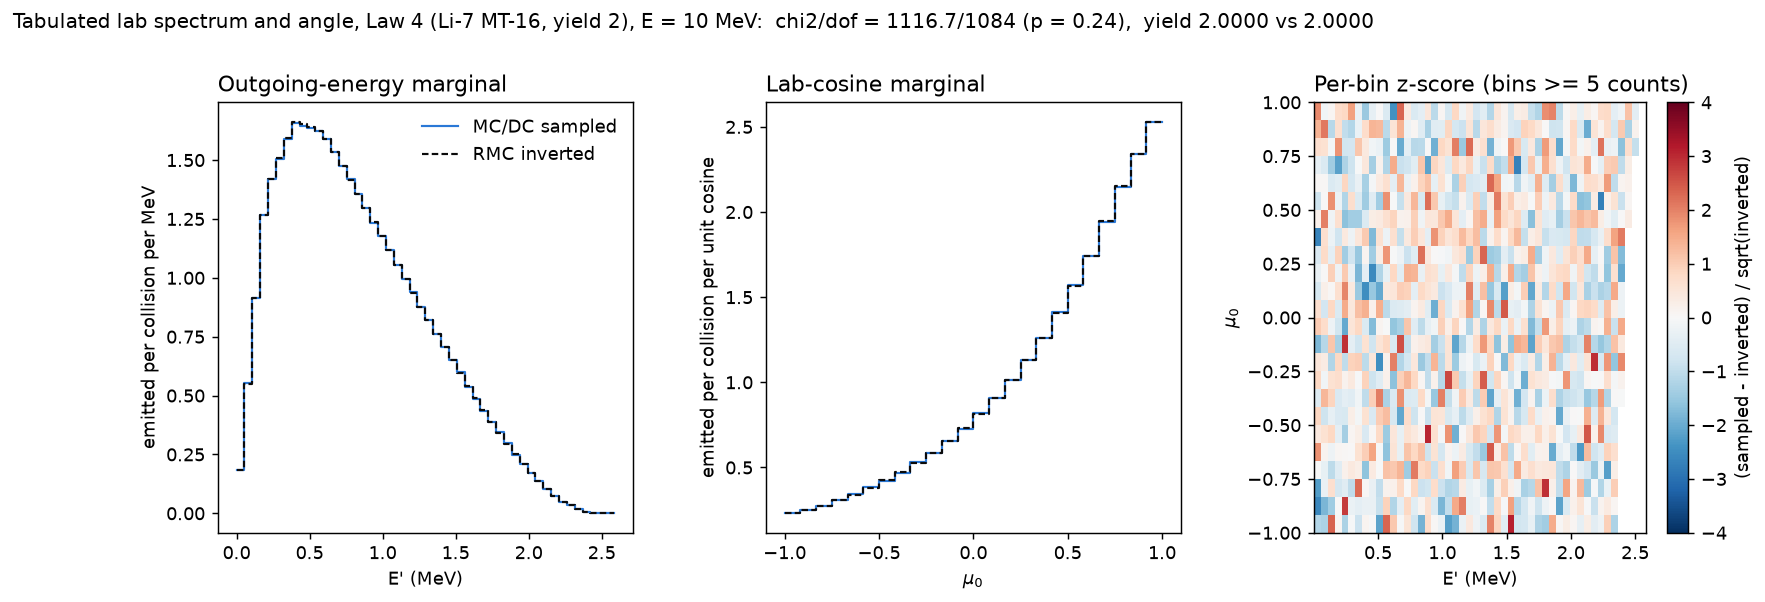
\includegraphics[width=\textwidth]{figures/tabulated/tabulated_E1e07.png}
  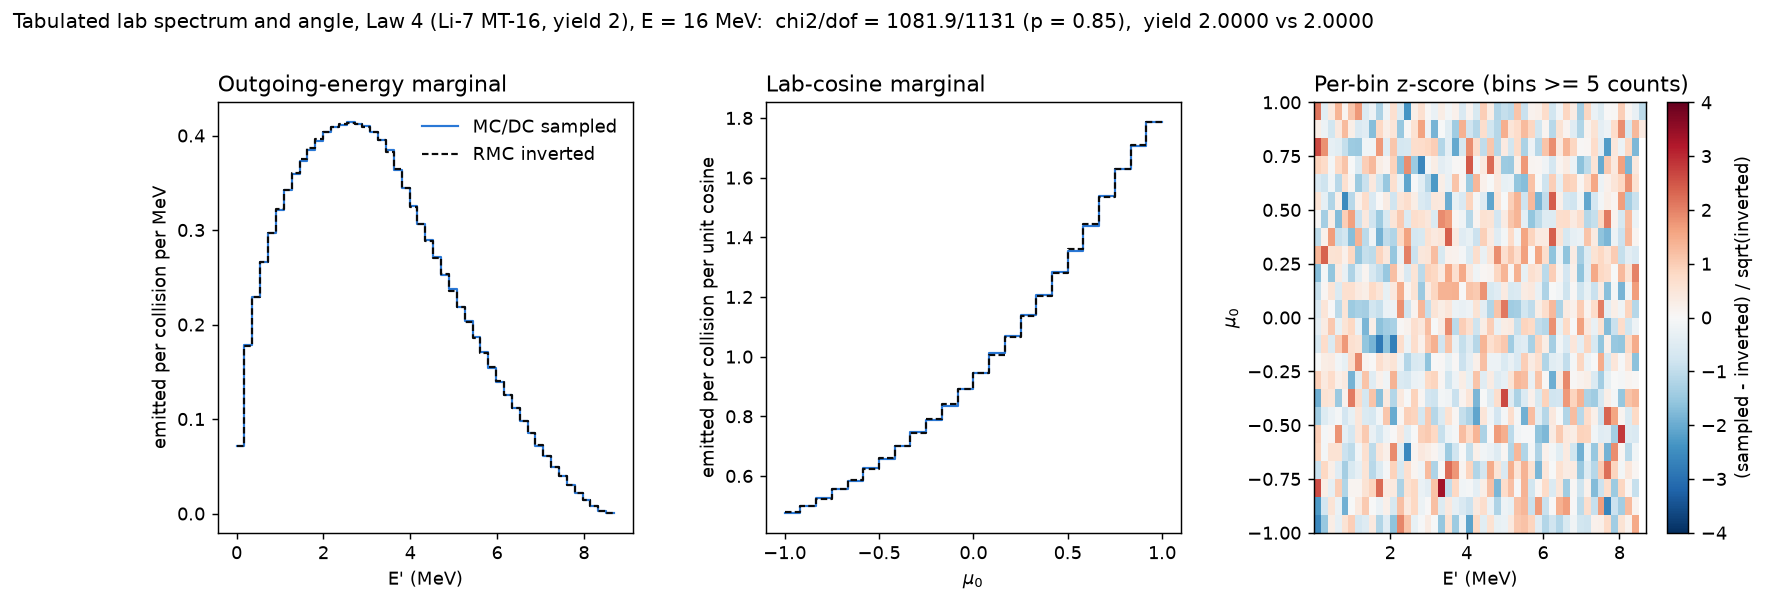
\includegraphics[width=\textwidth]{figures/tabulated/tabulated_E1p6e07.png}
  \caption{Li-7 MT-16 $(n,2n)$, a lab-frame tabulated energy spectrum with tabulated
  angular distributions, at 10 and 16\,MeV; two neutrons per collision.}
\end{figure}

\begin{figure}[h]
  \centering
  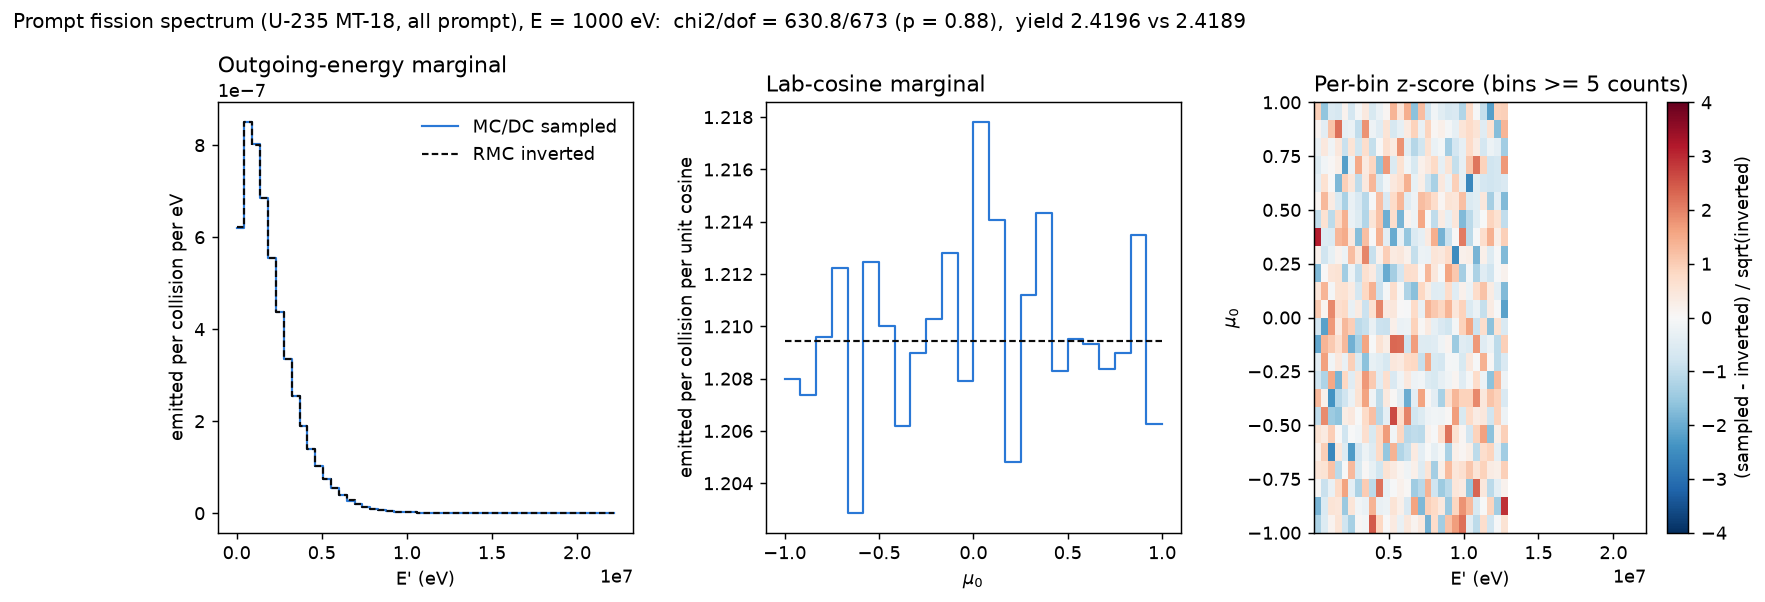
\includegraphics[width=\textwidth]{figures/fission/fission_E1000.png}
  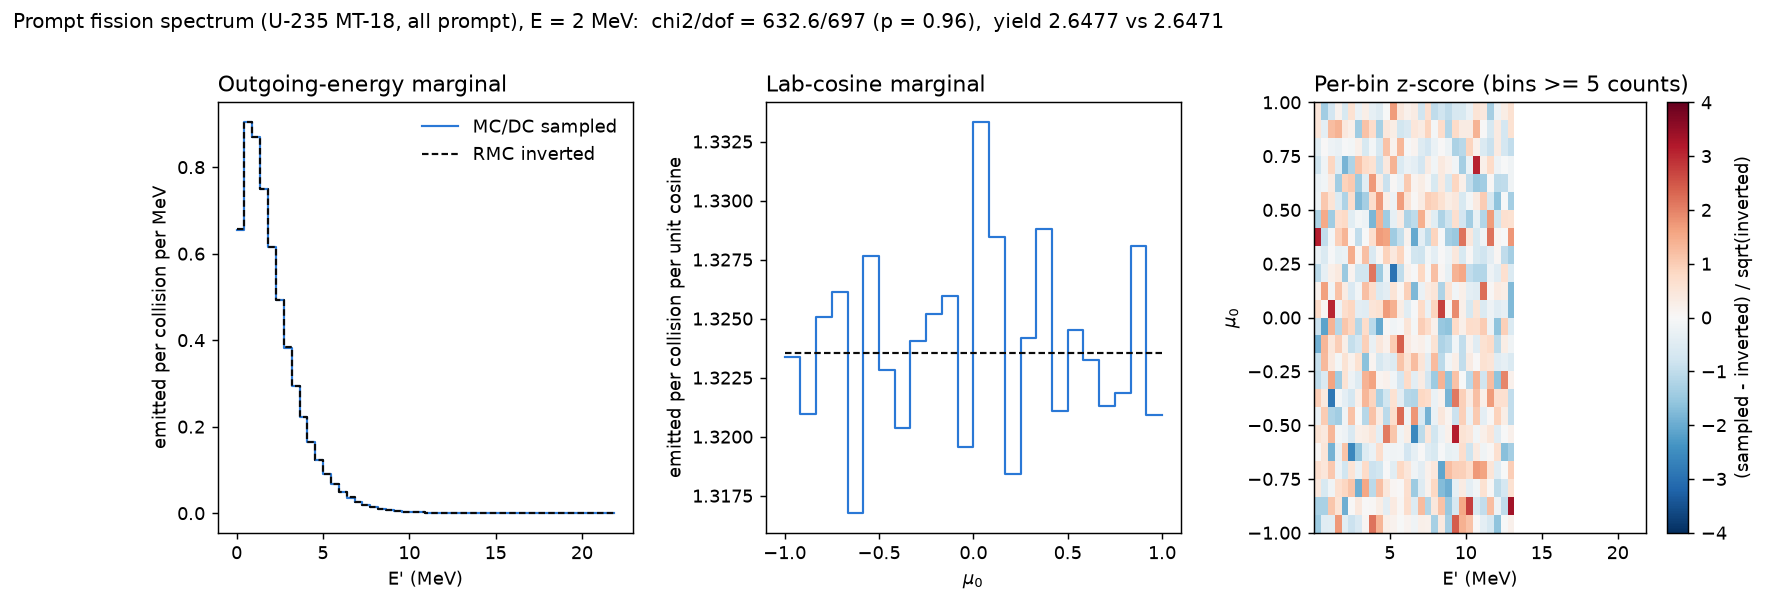
\includegraphics[width=\textwidth]{figures/fission/fission_E2e06.png}
  \caption{U-235 prompt fission spectrum at 1\,keV and 2\,MeV (isotropic lab
  emission). The yield column compares the sampled neutrons per fission with
  $\nu(\Ein)$.}
\end{figure}

\end{document}
